% by Razieh Pourhasan
\section{Applications to Time Series} \label{Section:5}
%\subsection{Application in finance }
In this section outliers and anomalies in time series are briefly discussed. A time series is the sequential set of values tracked over a time duration. R provides lots of packages with different approaches for detecting outliers and anomalies in time series. Here, two of the most commonly used are introduced and applied to a time series data. \subsection{Outliers and anomalies in time series} \textbf{Outliers in time series} are often sudden changes in the dynamics of the data that can be temporary or permanent. These changes are usually inconsistent with the rest of the series and cannot be explained by standard time series models. If not treated, they have an impact on the analysis such as model selection and parameter estimations. Therefore, they affect the forecasting power of the fitted model. Then it is important to detect and treat outliers in time series before fitting a model. \par Outliers that only change the mean level of the series are called deterministic. A simple procedure to detect deterministic outliers in time series is to compare a time series model with no outliers to another model that includes outliers \cite{tsay}. Estimates of the effect of treating any outliers is then given by the differences between the models. \par In general, detecting outliers in applied time series consists of determining the location, type, and magnitude of any existing outliers. There are several types of outliers as listed below: 
\begin{itemize}[noitemsep]
\item \textbf{Additive Outlier (AO)} is an abrupt change for only one observed value. Such an outlier has no effect on the subsequent observations. It is called a \textbf{seasonal additive outlier} when an additive outlier appears repeatedly at regular intervals.
\item \textbf{Innovational Outlier (IO)} is an unsual innovation\footnote{The \textit{innovations} in time series are used in the same way as \textit{errors} in cross-sectional analysis (such as OLS). Perhaps, the reason it is called \textit{innovation} is that it brings new information into time series data and it is new in the sense that observations are timely ordered.} in the generating process that affects all later observations. The influence of the outliers may increase with time.
\item \textbf{Level Shift Outlier (LS)} affects the mean level of observations so that all the observations after the outlier shift to a new level. Clearly such outliers have a permanent effect on the time series, therefore it is important to detect and treat them prior to building any forecasting model. It is called \textbf{seasonal level shift (SLS)} if the shift in the mean level occurs at regular intervals.
\item \textbf{Transient Change Outlier (TC)} is similar to level shift outlier but its effect is not permanent rather disappears over subsequent observations. That is, the time series returns to its normal level after a transient shift.
\end{itemize}
\textbf{Anomalies} are essentially the outliers. Things that happen regularly in the series are trend. However, observations that occur not often and are deviant from the regular pattern or trend in the series are anomalies.
The rest of this section is devoted to application of R packages, and functions therein, to detect outliers and anomalies. 
\subsection{R package: tsoutliers} The package \verb|tsoutlier| automatically detects outliers in time series based on the procedure proposed by Chen and Liu (1998) \cite{chenliu}. In this approach, the outlier effects are estimated simultaneously using multiple ARIMA based regression, and the model parameters and the outlier effects are estimated jointly. \par The main interface to the automatic detection procedure is through the funtion \verb|tso(x, types)|, where \verb|x| is a time series object and \verb|types| is a character vector indicating the type of outliers to be considered by the procedure. All five types of outliers described in the previous section can be considered; \verb|AO|, \verb|IO|, \verb|LS|, \verb|LSL| and \verb|TC|. If \verb|types| is not specified \verb|AO|, \verb|LS| and \verb|TC| would be considered by default. \par \textbf{Example: DJ30\footnote{The DJ30 consists of 30 stocks that are meant to reflect US market performance.}.} historical data of all stocks currently involved in the Dow Jones Industrial Average is available online on Kaggle \cite{dj30}. For each of the 30 components of the index, there is one CSV file named by the stock's symbol (e.g. AAPL for Apple Inc.). Each file provides historically adjusted market-wide data (daily, max. 5 years back). After reading all the CSV files with \verb|read.csv| function in R, the daily closing return for each component has been sorted by date and stored in a data frame named \verb|data|. The package \verb|tsoutliers| has been downloaded and outliers for Apple Inc. has been identified with the help of \verb|tso| function:
\begin{lstlisting}[language=R]
tso(ts(data$AAPL), 
       types=c("TC","AO","LS","IO","SLS"))
\end{lstlisting}
The output is a list type consisting of \verb|Coefficients| and \verb|Outliers|. The following is the R output for outliers of Apple Inc. data:
\begin{lstlisting}[language=R]
Outliers:
   type  ind time coefhat  tstat
1    TC  159  159   4.040  4.074
2    AO  302  302  -6.116 -4.405
3    AO  305  305   5.735  4.130
4    AO  410  410  -6.571 -4.732
5    TC  473  473  -4.521 -4.560
6    AO  536  536   6.496  4.678
7    AO  666  666   6.098  4.392
8    AO  791  791   6.629  4.774
9    AO 1043 1043   5.891  4.243
10   AO 1109 1109  -6.633 -4.777
11   AO 1144 1144   7.042  5.072
12   AO 1149 1149  -9.961 -7.174
13   AO 1167 1167   6.833  4.921
14   AO 1238 1238  -5.812 -4.186
\end{lstlisting}
There are 14 outliers with two being of \textit{transient change} type while the rest are \textit{additive outliers}. The outliers has been also illustrated in Figure~\ref{fig:apoutlier}; 
\begin{figure}[t]
\centering
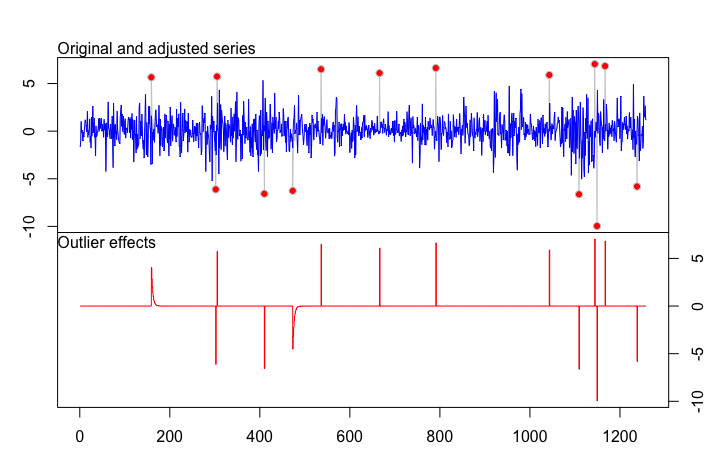
\includegraphics[width=0.30\textwidth]{\MainFolder/Images/Apoutliers.png}
\caption[\small Outliers detection for Apple Inc. daily closing return]{\small Outliers detection for Apple Inc. daily closing return. The x-axis is labelled by the date index.}
\hrule\label{fig:apoutlier}
\end{figure}
\afterpage{\FloatBarrier}
The isolated sharp spikes represent \textit{additive outliers} while a spike that takes a few periods to disappear represents a \textit{transient change oulier}. Also, note that the x-axis has been labelled by the time(date) index not the actual date. However, the actual date can be easily obtained. In the following R code the date of each output has been extracted where the output of the above \verb|tso| function has been saved as \verb|out_tso|:
\begin{lstlisting}[language=R]
ots=out_tso$outliers
cbind.data.frame(type=ots$type,date=data[ots$ind,1])
\end{lstlisting}
and the output is:
\begin{lstlisting}[language=R]
   type       date            type       date
1    TC 2015-01-28        8    AO 2017-08-01
2    AO 2015-08-21        9    AO 2018-08-01
3    AO 2015-08-26       10    AO 2018-11-02  
4    AO 2016-01-27       11    AO 2018-12-26
5    TC 2016-04-27       12    AO 2019-01-03
6    AO 2016-07-27       13    AO 2019-01-30
7    AO 2017-02-01       14    AO 2019-05-13
\end{lstlisting}


\subsection{R package: anomalize} Anomaly Detection is helpful for every marketer to keep an eye on company’s growth. For the marketing purpose, it is also better to do anomaly detection on a daily basis so that it helps the marketer to find the reason behind it and also to fix it as soon as possible. In this section the package \verb|anomalize| is used to detect anomalies in a time series data. The package is available on CRAN, then the stable version can be installed directly from there. However, the latest development of the package is available on github. Therefore it is recommended to first install the package from CRAN so that the dependencies are also installed then update the package using devtools as shown in the code below:

\begin{verbatim}
install.packages('anomalize')
library(devtools)
install_github("business-science/anomalize")
library(anomalize)
\end{verbatim}

The \verb|anomalize()| function in the package is used to detect outliers in a distribution with no trend or seasonality present while using \verb|tidyverse|\footnote{That package needs to be installed too.}. The return has three columns: "remainder-l1" (lower limit for anomalies), "remainder-l2" (upper limit for anomalies), and "anomaly" (Yes/No). The first argument of the function is \verb|data| which is a \verb|tibble| or \verb|tbl_time| object. The second argument \verb|target| is a column to apply the function to, and \verb|method| is the anomaly detection method which can be one of "iqr" or "gesd". 
\par The \textbf{IQR method} (Inner Quartile Range) takes a distribution and uses the 25\% and 75\% inner quartile range to establish the distribution of the remainder. Limits are set by default to a factor of 3X above and below the inner quartile range, and any remainders beyond the limits are considered anomalies. The alpha parameter adjusts the 3X factor. By default, alpha = 0.05 for consistency with the GESD method. An alpha = 0.025, results in a 6X factor, expanding the limits and making it more difficult for data to be an anomaly. Conversely, an alpha = 0.10 contracts the limits to a factor of 1.5X making it more easy for data to be an anomaly. The IQR method does not depend on any loops and is therefore faster and more easily scaled than the GESD method. However, it may not be as accurate in detecting anomalies since the high leverage anomalies can skew the centerline (median) of the IQR. \par The \textbf{GESD method} (Generlized Extreme Studentized Deviate Test) progressively eliminates outliers using a Student's T-Test comparing the test statistic to a critical value. Each time an outlier is removed, the test statistic is updated. Once test statistic drops below the critical value, all outliers are considered removed. The alpha parameter adjusts the width of the critical values. By default, alpha = 0.05. Because this method involves continuous updating via a loop, it is slower than the IQR method. However, it tends to be the best performing method for outlier removal. \par The remaining arguments in \verb|anomalize()| are \verb|alpha|, 
\verb|max_anoms| and \verb|verbose|; the parameter \verb|alpha| which is used in IQR method controls the width of the "normal" range. Lower values are more conservative while higher values are less prone to incorrectly classifying "normal" observations. \verb|max_anoms| is the maximum percent of anomalies permitted to be identified and \verb|verbose| is a boolean. If TRUE, will return a list containing useful information about the anomalies. If FALSE, just returns the data expanded with the anomalies and the lower (l1) and upper (l2) bounds. \par \textbf{Example DJ30-continue.} in the previous section function \verb|tsoutliers| was used to detect outliers of daily closing return for one of the components of DJ30, i.e. Apple Inc. An alternative would be anomaly detection using \verb+anomalize+ which can be done using the following R code: 
\begin{lstlisting}
data_tb=data %>% as.tibble()
data_tb %>% 
  time_decompose(AAPL,
                 method="stl",
                 frequency=10,
                 trend="auto") %>%
  anomalize(remainder,
            method="gesd",
            alpha=0.05,
            max_anoms=0.2) %>%
  plot_anomaly_decomposition()
\end{lstlisting}

The output is shown in Figure~\ref{fig:apanomalies}.
\begin{figure*}[H]
\centering
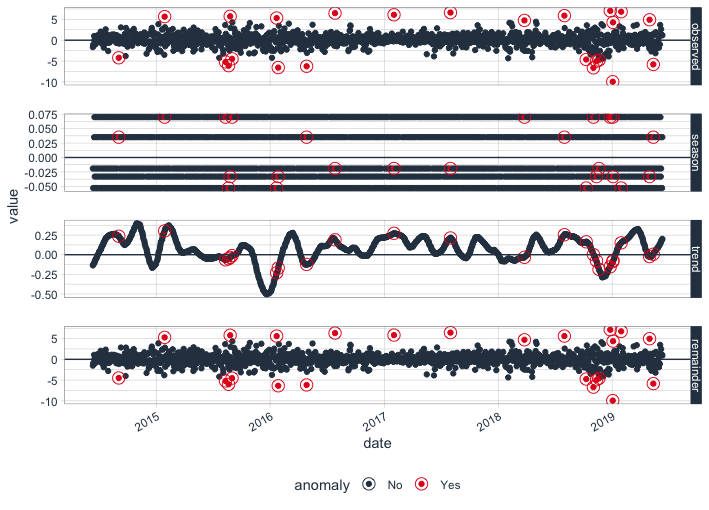
\includegraphics[width=0.5\textwidth]{\MainFolder/Images/Apanomalies.png}\label{fig:apanomalies}
\caption[\small Anomaly detection for Apple Inc. daily closing return]{\small Anomaly detection for Apple Inc. daily closing return.}
\hrule
\end{figure*}
\afterpage{\FloatBarrier}
where the top plot is overall observed data, followed by the season and trend and finally the bottom plot is detecting anomalies. The red points in each plot indicate anomalies according to the \verb|anomalize| function.  The series can also be plotted with recomposed data with \verb|time_recomposed()| function using the following code:
\begin{verbatim}
data_tb %>% time_decompose(AAPL) %>% 
  anomalize(remainder) %>% 
  time_recompose() %>%  
  plot_anomalies(time_recomposed=TRUE,
                 ncol=3,
                 alpha_dots=0.5)
\end{verbatim}
The output is shown in Figure~\ref{fig:apanomaliesrecomp}.
\begin{figure*}[H]
\centering
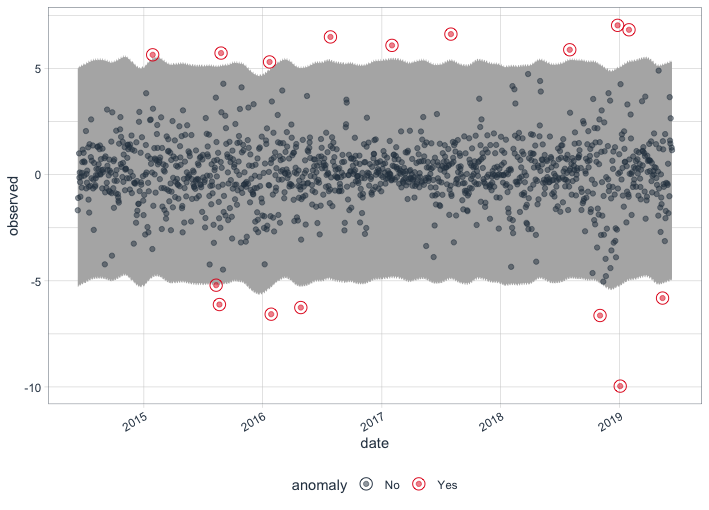
\includegraphics[width=0.5\textwidth]{\MainFolder/Images/Apanomaliesrecomp.png}
\caption[\small Anomaly detection for Apple Inc. daily closing return with recomposed data]{\small Anomaly detection for Apple Inc. daily closing return with recomposed data. The grey portion explains the expected trend.}
\hrule\label{fig:apanomaliesrecomp}
\end{figure*}

\afterpage{\FloatBarrier}
Further, anomaly points that are shown in red can be extracted by the following code:

\begin{verbatim}
anomalies=data_tb %>%  
time_decompose(AAPL) %>%  
 anomalize(remainder) %>%  
 time_recompose() %>%  
 filter(anomaly=='Yes')
\end{verbatim}

The output is a time tibble with 16 rows of 10 variables with \verb|date| and \verb|observed| being the first two variables. Therefore \verb|anomalize| reports 16 observations as anomalies. Recall that in previous section, \verb|tsoutliers| detected 14 outliers. It is interesting to compare the outlier/anomaly dates for Apple Inc. data from both approaches. This can be done with the code below:
\begin{lstlisting}
odates=cbind.data.frame(type=ots$type,
                 date=data[ots$ind,1])
adates=cbind.data.frame(date=anomalies$date,
                observed=anomalies$observed)
left_join(adates,odates,by="date")
\end{lstlisting}
Here is the result:
\begin{lstlisting}
        date observed type
1  2015-01-28    5.653   TC
2  2015-08-11   -5.204 <NA>
3  2015-08-21   -6.116   AO
4  2015-08-26    5.735   AO
5  2016-01-22    5.317 <NA>
6  2016-01-27   -6.571   AO
7  2016-04-27   -6.258   TC
8  2016-07-27    6.496   AO
9  2017-02-01    6.098   AO
10 2017-08-01    6.629   AO
11 2018-08-01    5.891   AO
12 2018-11-02   -6.633   AO
13 2018-12-26    7.042   AO
14 2019-01-03   -9.961   AO
15 2019-01-30    6.833   AO
16 2019-05-13   -5.812   AO
\end{lstlisting}
It is clear that all the points that have been detected by \verb|tsoutliers| match the ones reported by \verb|anomalize|. However, \verb|anomalize| detect two extra points which are missing in \verb|tsoutliers| output, that's why the type is not specified for these two points. The comparison is also illustrated in Figure~\ref{fig:comparemethods}.
\begin{figure}[t]
\centering
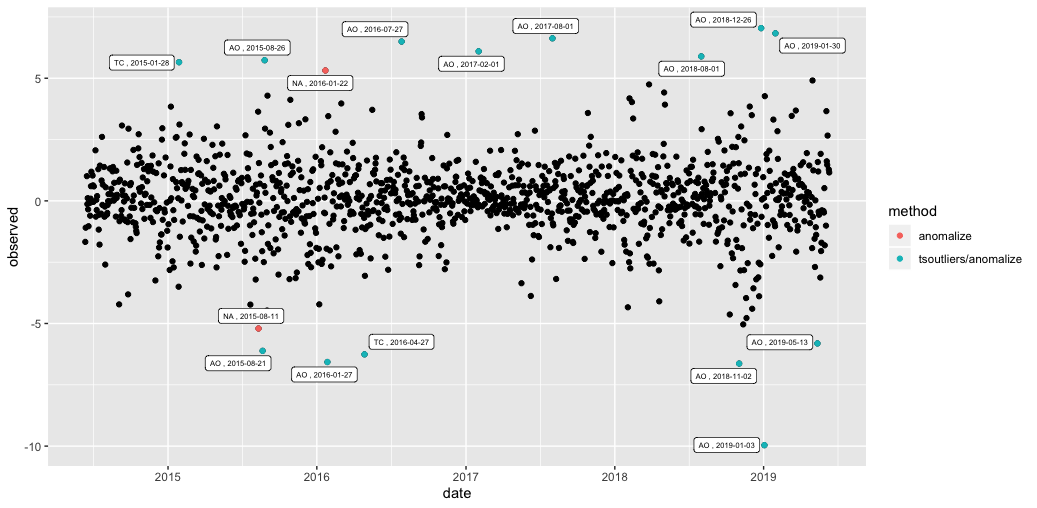
\includegraphics[width=0.5\textwidth]{\MainFolder/Images/comparemethods.png}
\caption[\small Comparing two methods of outlier/anomaly detection for Apple Inc. daily closing return.]{\small Comparing two methods of outlier/anomaly detection for Apple Inc. daily closing return.}
\hrule\label{fig:comparemethods}
\end{figure}
\afterpage{\FloatBarrier}

\subsection{Summary}
In many disciplines outlier detection is critical but it is even more important in marketing analysis where data are often in forms of time series.  Since in marketing, outliers are often visible symptoms of underlying problems that need to be fixed fast. In this section two R packages were reviewed where each uses different approach to automatically detect outliers: \verb|tsoutliers| and \verb|anomalize|, and their outputs were compared on a selected time series . The definition that is used in each approach to detect outliers is simple: an outlier is essentially something that occurs unexpectedly or caused by an abnormal event. Therefore, the problem of finding outliers is providing methods to accurately detect these \textit{anomalous} events. \par For time series data, anomaly detection is usually performed on \textbf{remainders} of a time series where both \textbf{seasonal} and \textbf{trend} components were removed; the former is the presence of variations that occur at specific regular intervals less than a year, such as daily, weekly, monthly, or quarterly while the later is longer term growth that happens over many observations. Thus the first task in anomaly detection is to generate remainders from a time series. \par There are different ways to decompose a time series to produce remainders such as ARIMA, machine learning (regression), seasonal decomposition, and so on. The package \verb|tsoutliers| uses ARIMA while \verb|anomalize| uses seasonal decomposition. In general, high performance machine learning techniques are not recommended for anomaly detection since the overfitting reduces the difference between the observed and fitted values where as in anomaly detection this difference is essential to highlight the anomaly. On the other hand, seasonal decomposition performs best for this task by removing the right features (i.e. seasonal and trend components) while preserving the characteristics of anomalies in the remainders. \par As final remark, there is another popular package in R, i.e., \verb|AnomalyDetection| developed by Twitters that is not reviewed here. However, the approach used there is similar to method \textit{GESD} in \verb|anomalize|. Interested reader is invited to try this package and functions therein and compare their results with other functions introduced in this section. 

%\subsection{More applications}
